% =============================================================================
%  Into Frame -- project report
%
%  Build:   latexmk -pdf main.tex
%  or:      pdflatex main && bibtex main && pdflatex main && pdflatex main
%
%  Body text lives in sections/, pulled in by the \input list below -- edit those
%  files, not this one. This file holds only the preamble, the title block and
%  the bibliography.
%
%  Figures live in figures/ and are included through \figbox (see below), so the
%  document compiles cleanly before any of them exist.
% =============================================================================
\documentclass[11pt,a4paper]{article}

\usepackage[T1]{fontenc}
\usepackage[utf8]{inputenc}
\usepackage{lmodern}
\usepackage[margin=2.4cm]{geometry}
\usepackage{graphicx}
\usepackage{booktabs}
\usepackage{amsmath}
\usepackage{amssymb}
\usepackage{siunitx}
\usepackage{microtype}

\linespread{0.8}
\usepackage{caption}
\usepackage{subcaption}
\usepackage{enumitem}
\usepackage{xcolor}
\usepackage[hidelinks]{hyperref}
\usepackage{cleveref}
\usepackage{tikz}
\usetikzlibrary{arrows.meta,positioning,fit,backgrounds}

\graphicspath{{figures/}}

% -----------------------------------------------------------------------------
% Placeholder handling: \figbox{file}{alt-text}{width} draws a framed placeholder
% when figures/<file> is missing, so the document always builds. Drop the real
% image into figures/ and it is picked up automatically.
% -----------------------------------------------------------------------------
\newcommand{\figbox}[3]{%
  \IfFileExists{figures/#1}%
    {\includegraphics[width=#3\linewidth]{#1}}%
    {\fbox{\parbox[c][0.26\textheight][c]{#3\linewidth}{\centering\ttfamily\small
      [figure placeholder]\\[2pt] figures/#1\\[6pt]\normalfont\itshape #2}}}%
}

\sisetup{detect-weight=true, detect-family=true}

\title{\textbf{Jumping Into the Frame}\\[0.4em]
\large Reconstructing Interactive, Physically-Grounded 3D Environments\\
from a Single Image}

\author{Joshua Ford \\
\textbf{Advisor:} Marie-Paule Cani}
\date{\today}

\begin{document}
\maketitle

\begin{abstract}
\noindent
Single-image 3D scene generation has advanced rapidly, but most systems stop at a
viewable, inert result: a panorama, a layered mesh, or a radiance field that
supports novel-view synthesis but has no motion and nothing to interact with.
We present \textbf{Into Frame}, a system that turns one photograph into an
\emph{inhabitable} environment, in which discrete objects exist as individual
simulated assets, ground cover and vegetation respond to contact and wind, and
the scene is lit by a physically based estimate of the original illumination, all
at real-time VR frame rates.
Our central design commitment is to reconstruct each part of the scene by a
method suited to its physical role, rather than extracting everything from one
representation: terrain, objects, ground cover, water and sky are handled
separately and by different means.
We outline the pipeline built on this principle and focus on four contributions:
a projection from calibrated panoramic depth to a top-down height field that
preserves each cell's observed panorama pixel; a terrain reconstruction that
keeps visual similarity with the original image while applying fluvial erosion to
give plausible relief where nothing was observed; a pattern-texturing scheme that
avoids the projective smearing an equirectangular photograph produces on the
ground; and a point-process population synthesis that scatters vegetation and
objects to match the spatial statistics of the real detections.
We evaluate the system on several real-world images and report both what it does
well and a set of failure modes we were able to measure precisely. We argue that
the most transferable result is methodological: at this scale, most defects are
not model failures but \emph{assumption} failures, where a step valid for one
scene category is silently applied to another.
\end{abstract}


% -- body ---------------------------------------------------------------------
% Comment out any line to build a subset while drafting; cross-references into a
% dropped section will warn but still compile.
% =============================================================================
\section{Introduction}
% =============================================================================

\subsection{Motivation}

A photograph is a two-dimensional projection of a three-dimensional world, and
recovering that world from a single view is underconstrained: infinitely many
scenes project to the same image.
Humans nonetheless read a photograph as a place. We infer that the ground
continues past the frame, that the occluded side of a rock exists, that the
flowers in the foreground are individual plants rather than a printed texture.
Building an environment that supports those inferences, one a person can
\emph{jump into}, is the problem this project begins to address.

Photographs are among the most abundant records of place we have: personal
archives, cultural heritage documentation, scientific field imagery, and now,
with generative models, images of places that never existed at all. A system that
converts such an image into an environment a person can walk into changes what
those archives are able to express. It also lowers the cost of 3D content
authoring by several orders of magnitude relative to manual modeling or
multi-view capture, and because the process is automatic, it puts that authoring
within reach of a non-expert.

\subsection{The Challenge}

The difficulty is not one hard sub-problem but the interaction of several, each
of which degrades the others:

\begin{description}[leftmargin=1.2em,style=nextline]
  \item[Extreme ill-posedness.] A single view fixes neither absolute scale nor
  the geometry of anything it does not see. Roughly $5/6$ of a full
  $360^\circ$ panorama generated from a standard photograph is synthesized rather
  than observed, and everything behind every foreground object is unknown. Much
  of the world must be inferred.

  \item[Compounding error.] A pipeline that estimates depth, then geometry, then
  materials, then objects inherits every earlier error, and a discrepancy that is
  barely visible at one stage can be structural by the next.

  \item[Heterogeneous content.] The representation that suits a mountainside
  (a height field) is wrong for a tree (a mesh instance), which is wrong for a
  meadow (a scattered population), which is wrong for the sea (an animated
  surface). These representations must nonetheless coexist in one scene: they
  need to share a coordinate frame and a scale, agree on how they are lit, and
  not seam visibly where they meet.

  \item[Interactivity constraints.] The output must render stereoscopically at
  headset frame rates. That budget constrains every rendering choice, and it
  binds hardest on the animated, simulated elements that make the scene
  interactive in the first place.

\end{description}

\subsection{Goals}

Our goal is a system that takes one image and produces an environment which is
\emph{interactive} (objects animate and interact with their surroundings),
\emph{decomposed} (discrete objects exist as individual entities, not painted
texture), \emph{plausible} beyond the observed region, and \emph{performant} at
VR frame rates.

% =============================================================================
\section{Related Work}
\label{sec:related}
% =============================================================================

\subsection{Single-Image Panorama Generation}

Extending a narrow-field photograph to a full $360^\circ$ environment is the
first step in most single-image scene systems. Diffusion models adapted to
panoramic geometry are the dominant approach.
CubeDiff~\cite{kalischek2025cubediffrepurposingdiffusionbasedimage} repurposes a
perspective latent diffusion model for panorama generation by operating on
cubemap faces with synchronized attention.
DreamCube~\cite{dreamcube,dreamcube_arxiv} extends this to RGB-D panoramas
through multi-plane synchronization, producing geometry alongside appearance.
PanoDreamer~\cite{paliwal2024panodreamer} takes an optimization-based route to
coherent single-image $360^\circ$ scenes, and
LayerPano3D~\cite{yang2024layerpano3d} decomposes the panorama into depth layers
to support larger viewpoint changes.
Our system supports several such backends, defaulting to a
FLUX-based~\cite{esser2024scalingrectifiedflowtransformers} outpainting path,
with WorldGen~\cite{worldgen2025ziyangxie} and DreamCube as alternatives. The
relevant distinction is that we treat the panorama as an intermediate
representation rather than as the deliverable.

\subsection{Single-Image 3D Scene Generation}

A growing body of work targets navigable 3D scenes from one image.
SphericalDreamer~\cite{schnepf2026sphericaldreamer} generates navigable immersive
worlds; SonoWorld~\cite{jin2026sonoworld} extends single-image scene generation to
audio-visual output; 360Anything~\cite{wu360anything} lifts images and videos
to $360^\circ$ geometry-free representations; and
WorldGen~\cite{worldgen2025ziyangxie} produces complete 3D scenes rapidly.
These systems generally optimize for visual fidelity from viewpoints near the
original camera. Into Frame instead prioritizes \emph{physical decomposition}: the
output is not one geometry proxy but a set of typed entities with distinct
behavior, a collidable terrain mesh, individually placed object meshes, an
instanced ground-cover population and an animated water surface. Each is required
before a scene can be dynamic rather than merely viewable.

\subsection{Depth Estimation and Panoramic Depth}

Monocular depth estimation underpins all geometry in the pipeline. We use
Depth Anything 3~\cite{lin2025depth3recoveringvisual} for perspective depth and
Depth Any Panoramas~\cite{lin2025dap} for equirectangular depth, the latter
avoiding the distortion artifacts that arise when a perspective model is applied
to equirectangular imagery. A recurring difficulty, which we address explicitly
in \cref{sec:panorama}, is that monocular depth is relative and saturates: real
distant terrain and sky receive indistinguishable predictions, so calibrated depth
at a ridge crest is an extrapolation rather than a measurement.

\subsection{Terrain Modeling and Heightmap Synthesis}

Recovering terrain from imagery connects to a long line of graphics work.
Pixels2Peaks~\cite{jain:hal-05617061} converts terrain images to heightmaps
directly; terrain modeling from feature primitives~\cite{genevaux:hal-01257198}
builds terrain from sparse user-specified features;
Earthbender~\cite{10.1145/3769047.3769053} offers interactive stylistic heightmap
generation; and WorldBrush~\cite{10.1145/2766975} synthesizes procedural worlds
from examples, including the distribution of scene elements. For physical
plausibility of unobserved relief we use
Landlab~\cite{barnhart2020landlab,hobley2017creative,Hutton_landlab_2020}, an
Earth-surface dynamics toolkit, applying fluvial incision so that invented terrain
obeys drainage structure rather than reading as smooth interpolation or undirected
noise.

\subsection{Texture Synthesis}

Projecting a panorama onto ground fails at grazing incidence: a single panorama
row covers meters of ground at distance. Pattern-based
texturing~\cite{neyret:inria-00537511} addresses exactly this class of problem by
assembling surfaces from patterns rather than resampling a projection, and our
terrain texturing follows that idea using patches extracted from the real
photograph. Where synthetic material is unavoidable we use
FLUX~\cite{esser2024scalingrectifiedflowtransformers} and latent diffusion
models~\cite{Rombach_2022_CVPR}, with
Swin2SR~\cite{conde2022swin2srswinv2transformercompressed} for super-resolution.

\subsection{Segmentation, Detection and Recognition}

Object decomposition uses SAM~2~\cite{ravi2024sam2segmentimages} for segmentation
and video tracking, Grounding DINO~\cite{liu2024groundingdino} for
open-vocabulary detection and label verification,
CLIP~\cite{radford2021learningtransferablevisual} for embedding-based
classification,
BLIP~\cite{li2022blipbootstrappinglanguageimagepretraining} and
Florence-2~\cite{xiao2024florence2} for captioning,
Recognize Anything~\cite{zhang2023recognize,huang2023tag2text} and its open-set
successor RAM++~\cite{huang2023open} for scene tagging,
SegFormer~\cite{DBLP:journals/corr/abs-2105-15203} for semantic region typing, and
BiRefNet~\cite{zheng2024birefnet} for high-resolution matting. Each solves a
similar but subtly different problem; we combine them rather than choosing between
them, using their agreement where they overlap to build a more reliable reading of
the scene than any one provides alone.

\subsection{Object Reconstruction and Inpainting}

Individual objects are reconstructed with
SAM~3D~\cite{sam3dteam2025sam3d3dfyimages}, with
SPAR3D~\cite{huang2025spar3dstablepointawarereconstruction} and
TRELLIS~\cite{xiang2025trellis2} as alternatives.
Removing foreground objects so the ground behind them can be reconstructed uses
inpainting: LaMa~\cite{suvorov2021resolution},
MAT~\cite{li2022mat}, Inpaint Anything~\cite{yu2023inpaint}, and
ObjectClear~\cite{zhao2026objectclear}, the last targeting removal of both objects
and their effects.

\subsection{Lighting}

Relighting reconstructed content so that it matches the original photograph
requires recovering the scene illumination. We use
LuxDiT~\cite{liang2025luxdit} for HDR lighting estimation
and IntrinsicDiffusion~\cite{Luo2024IntrinsicDiffusion} to separate albedo from
shading, so that assets carry material color rather than baked-in sunlight and
can be lit by our own lighting algorithm.

% =============================================================================
\section{Overview}
\label{sec:overview}
% =============================================================================

\begin{figure}[t]
  \centering
  % Wider than the text block: the diagram bleeds 0.9cm into each margin (which
  % are 2.4cm) so the stage labels stay legible. Change the 18cm to \linewidth
  % to keep it strictly inside the text block.
  \makebox[\linewidth][c]{\resizebox{18cm}{!}{% =============================================================================
%  Pipeline overview figure -- TikZ source.
%
%  Included from sections/03-method-overview.tex via \input. Requires, in the
%  preamble of main.tex:
%
%      \usepackage{tikz}
%      \usetikzlibrary{arrows.meta,positioning,fit,backgrounds}
%
%  Coordinates are in the units set by x=/y= below; the whole figure is about
%  19.5 x 9.0 units, so at 0.78cm/unit it lands close to \textwidth on A4 with
%  2.4cm margins. Change ONE number (the x=/y= scale) to resize everything.
%
%  Layout was prototyped and visually checked before being written out here;
%  every coordinate below is the one that was verified.
% =============================================================================
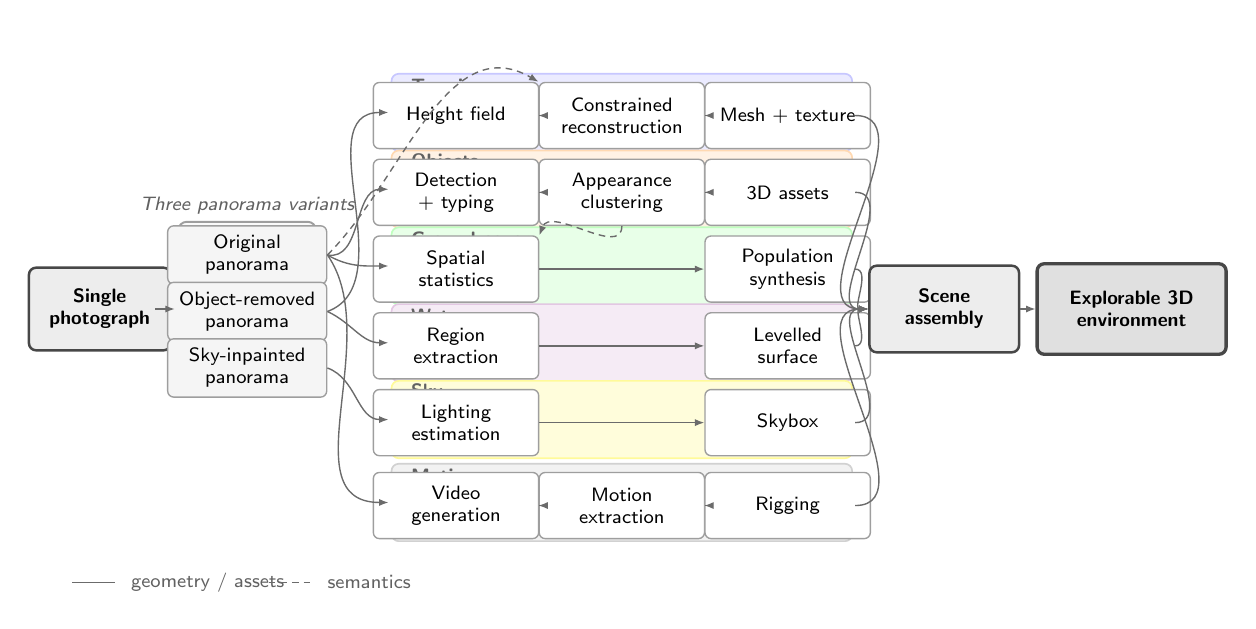
\begin{tikzpicture}[
  x=0.78cm, y=0.78cm,
  font=\sffamily,
  % ---- boxes -------------------------------------------------------------
  stage/.style={
    draw=black!38, line width=0.5pt, fill=white, rounded corners=2.2pt,
    align=center, inner sep=2.6pt, font=\sffamily\scriptsize,
    minimum width=2.10cm, minimum height=0.84cm},
  pano/.style={stage, fill=black!4, minimum width=2.02cm, minimum height=0.74cm},
  anchorbox/.style={
    draw=black!72, line width=0.9pt, fill=black!7, rounded corners=2.6pt,
    align=center, inner sep=3pt, font=\sffamily\scriptsize\bfseries},
  outbox/.style={anchorbox, line width=1.2pt, fill=black!12},
  % ---- containers --------------------------------------------------------
  panogroup/.style={
    draw=black!38, line width=0.7pt, fill=black!2, rounded corners=3pt},
  lanelabel/.style={
    anchor=west, font=\sffamily\scriptsize\bfseries, text=black!62},
  grouplabel/.style={font=\sffamily\scriptsize\itshape, text=black!62},
  % ---- edges -------------------------------------------------------------
  flow/.style={draw=black!58, line width=0.5pt, -{Latex[length=3.4pt,width=2.6pt]}},
  sem/.style={flow, dashed, dash pattern=on 2.4pt off 1.8pt},
]

% ---- lane backgrounds (drawn first, so boxes sit on top) -------------------
% one \filldraw per lane: fill, border, y-span
\filldraw[fill=blue!8,   draw=blue!22,   line width=0.6pt, rounded corners=2.6pt] (5.55, 5.67) rectangle (13.05, 6.93);
\filldraw[fill=orange!10, draw=orange!30, line width=0.6pt, rounded corners=2.6pt] (5.55, 4.42) rectangle (13.05, 5.68);
\filldraw[fill=green!9,   draw=green!25,  line width=0.6pt, rounded corners=2.6pt] (5.55, 3.17) rectangle (13.05, 4.43);
\filldraw[fill=violet!8,  draw=violet!22, line width=0.6pt, rounded corners=2.6pt] (5.55, 1.92) rectangle (13.05, 3.18);
\filldraw[fill=yellow!14, draw=yellow!40, line width=0.6pt, rounded corners=2.6pt] (5.55, 0.67) rectangle (13.05, 1.93);
\filldraw[fill=black!5,   draw=black!18,  line width=0.6pt, rounded corners=2.6pt] (5.55,-0.68) rectangle (13.05, 0.58);

\node[lanelabel] at (5.71,6.74) {Terrain};
\node[lanelabel] at (5.71,5.49) {Objects};
\node[lanelabel] at (5.71,4.24) {Ground cover};
\node[lanelabel] at (5.71,2.99) {Water};
\node[lanelabel] at (5.71,1.74) {Sky};
\node[lanelabel] at (5.71,0.39) {Motion};

% ---- input ----------------------------------------------------------------
\node[anchorbox, minimum width=1.80cm, minimum height=1.05cm] (photo) at (0.80,3.10)
  {Single\\photograph};

% ---- three panorama variants ----------------------------------------------
\draw[panogroup] (2.08,1.72) rectangle (4.32,4.52);
\node[grouplabel] at (3.20,4.78) {Three panorama variants};
\node[pano] (porig) at (3.20,3.98) {Original\\panorama};
\node[pano] (pterr) at (3.20,3.06) {Object-removed\\panorama};
\node[pano] (psky)  at (3.20,2.14) {Sky-inpainted\\panorama};

\draw[flow] (1.70,3.10) -- (2.02,3.10);

% ---- lane contents ---------------------------------------------------------
% three-step lanes: x = 6.60, 9.30, 12.00 ; two-step lanes: x = 6.60, 12.00
\node[stage] (t1) at (6.60,6.25) {Height field};
\node[stage] (t2) at (9.30,6.25) {Constrained\\reconstruction};
\node[stage] (t3) at (12.00,6.25) {Mesh + texture};
\draw[flow] (t1) -- (t2);   \draw[flow] (t2) -- (t3);

\node[stage] (o1) at (6.60,5.00) {Detection\\+ typing};
\node[stage] (o2) at (9.30,5.00) {Appearance\\clustering};
\node[stage] (o3) at (12.00,5.00) {3D assets};
\draw[flow] (o1) -- (o2);   \draw[flow] (o2) -- (o3);

\node[stage] (g1) at (6.60,3.75) {Spatial\\statistics};
\node[stage] (g2) at (12.00,3.75) {Population\\synthesis};
\draw[flow] (g1) -- (g2);

\node[stage] (w1) at (6.60,2.50) {Region\\extraction};
\node[stage] (w2) at (12.00,2.50) {Levelled\\surface};
\draw[flow] (w1) -- (w2);

\node[stage] (s1) at (6.60,1.25) {Lighting\\estimation};
\node[stage] (s2) at (12.00,1.25) {Skybox};
\draw[flow] (s1) -- (s2);

\node[stage] (m1) at (6.60,-0.10) {Video\\generation};
\node[stage] (m2) at (9.30,-0.10) {Motion\\extraction};
\node[stage] (m3) at (12.00,-0.10) {Rigging};
\draw[flow] (m1) -- (m2);   \draw[flow] (m2) -- (m3);

% ---- panorama -> lanes (geometry) -----------------------------------------
% which variant feeds which lane is the load-bearing detail; see the report text
\draw[flow] (pterr.east) to[out=20,in=180]  (5.50,6.30);   % object-removed -> terrain
\draw[flow] (porig.east) to[out=-10,in=180] (5.50,5.05);   % original       -> objects
\draw[flow] (porig.east) to[out=-30,in=180] (5.50,3.80);   % original       -> ground cover
\draw[flow] (pterr.east) to[out=-25,in=180] (5.50,2.55);   % object-removed -> water
\draw[flow] (psky.east)  to[out=-20,in=180] (5.50,1.30);   % sky-inpainted  -> sky
\draw[flow] (porig.east) to[out=-55,in=180] (5.50,-0.05);  % original       -> motion

% ---- semantics (dashed) ----------------------------------------------------
\draw[sem] (porig.east) to[out=45,in=150] (t2.north west);   % region typing -> ridge anchoring
\draw[sem] (o2.south)   to[out=-90,in=70] (g1.north east);   % exemplars     -> population stats

% ---- convergence -----------------------------------------------------------
\node[anchorbox, minimum width=1.90cm, minimum height=1.10cm] (asm) at (14.55,3.10)
  {Scene\\assembly};
\foreach \yy in {6.25, 5.00, 3.75, 2.50, 1.25, -0.10}
  { \draw[flow] (13.10,\yy) to[out=0,in=180] (asm.west); }

\node[outbox, minimum width=2.40cm, minimum height=1.15cm] (out) at (17.60,3.10)
  {Explorable 3D\\environment};
\draw[flow] (asm) -- (out);

% ---- legend ----------------------------------------------------------------
\draw[draw=black!58, line width=0.5pt] (0.35,-1.35) -- (1.05,-1.35);
\node[anchor=west, font=\sffamily\scriptsize, text=black!62] at (1.15,-1.35)
  {geometry / assets};
\draw[draw=black!58, line width=0.5pt, dashed, dash pattern=on 2.4pt off 1.8pt]
  (3.55,-1.35) -- (4.25,-1.35);
\node[anchor=west, font=\sffamily\scriptsize, text=black!62] at (4.35,-1.35)
  {semantics};

\end{tikzpicture}
}}
  \caption{The pipeline decomposes a single image into five tracks with different
  physical roles. Solid arrows carry geometry, dashed arrows carry semantics.
  The three panorama variants at the left are maintained deliberately: geometry is
  derived from the object-removed panorama, semantics from the original.}
  \label{fig:pipeline}
\end{figure}

\subsection{Design principle: role-specialised decomposition}

The organising commitment of Into Frame is that a scene is not one thing. Ground,
discrete objects, ground cover, water and sky differ in how they must be
reconstructed, how they are represented, how they are textured, and how they
behave at runtime. Forcing them through one representation means accepting the
weakest common denominator.

\Cref{fig:pipeline} shows the resulting structure. Concretely, the pipeline
maintains five tracks:

\begin{description}[leftmargin=1.2em,style=nextline]
  \item[Terrain.] A single continuous height field, meshed with variable density,
  carrying collision. Reconstructed from calibrated panoramic depth and completed
  by a constrained solve.
  \item[Objects.] Discrete entities detected, classified, clustered by visual
  similarity, and reconstructed once per (class, appearance) group, then instanced
  at every detection's position.
  \item[Ground cover.] Populations too numerous to place individually as
  reconstructions, scattered by density over a mask derived from semantics and
  colour.
  \item[Water.] Regions typed as water, extracted as a separate levelled surface
  with an animated shader.
  \item[Sky.] The panorama above the horizon, inpainted where objects were removed,
  used as both skybox and image-based lighting source.
\end{description}

\subsection{Execution model}

The pipeline comprises 40 active stages. Each declares typed inputs and outputs
against a shared \emph{context}, and each may report whether its output already
exists. When it does, the stage is skipped. A stage that runs marks everything
downstream dirty, so a rerun is a linear cascade from the earliest changed stage.

This is a development-time contribution as much as an engineering one. Full
pipeline execution takes hours, so the ability to invalidate one stage and rerun
only its consequences is what makes iteration possible at all. It also creates a
specific hazard we encountered repeatedly: a stage's cache-validity predicate must
mirror the conditions under which the stage itself would skip work. Where the two
diverge, the stage reports incomplete forever and every downstream stage reruns on
every invocation.

A second consequence is that the configuration file is not part of the cache key.
Changing a parameter therefore does not invalidate the stage it belongs to, and an
explicit rerun directive is required. This is a deliberate trade --- hashing
configuration would invalidate far more than necessary --- but it is a sharp edge.

\subsection{Stage sequence}

\Cref{tab:stages} groups the stages by track; \cref{sec:implementation} reports
what each costs to run. The ordering is not arbitrary:
several dependencies are counterintuitive and were established by failure. Object
segmentation runs on the \emph{original} panorama, before foreground inpainting,
because inpainting removes the objects that must be detected; but terrain geometry
is derived from the \emph{inpainted} panorama, because occluders would otherwise
punch holes in the ground. Maintaining both variants and routing each consumer to
the correct one is a recurring structural theme.

\begin{table}[t]
\centering
\small
\caption{Pipeline stages grouped by reconstruction track.}
\label{tab:stages}
\begin{tabular}{@{}llp{7.4cm}@{}}
\toprule
\textbf{Track} & \textbf{Stages} & \textbf{Purpose} \\
\midrule
Panorama    & 1--4   & Caption, perspective depth, $360^\circ$ outpainting, super-resolution \\
Semantics   & 5--8   & Panoramic depth, object segmentation, classification, typing \\
Cleanup     & 9--11  & Foreground removal, equirectangular LoRA correction \\
Regions     & 12--15 & Semantic region typing (original and object-removed), lighting estimation, sky inpainting \\
Geometry    & 16--19 & Panoramic depth, metric calibration, height field, region map \\
Terrain     & 20--25 & Constrained reconstruction, erosion refinement, meshing, texturing \\
Objects     & 26--30 & Recognition, detection, instance refinement, correlation, clustering \\
Population  & 31--33 & Spatial statistics, population synthesis, ground cover \\
Assembly    & 34--35 & Asset generation, scene assembly and placement \\
Animation   & 38--42 & Video generation, motion extraction, rigging, animation \\
\bottomrule
\end{tabular}
\end{table}

% =============================================================================
\section{The Panoramic Data}
\label{sec:panorama}
% =============================================================================

Every track in \cref{fig:pipeline} consumes the same three artifacts: a
$360^\circ$ panorama, an aligned metric depth map, and a per-pixel
semantic typing. The depth map and semantic typing are both derived from
the generated panorama, which extends the provided input image into a complete
$360^\circ$ view of the scene.

We use one capture, a photograph of Mount Rainier, as a running example throughout.
\Cref{fig:rainier-input} shows the input and the panorama generated from it: the
photograph covers roughly a sixth of the sphere, and everything else is synthesized.

\begin{figure}[htbp]
  \centering
  \begin{subfigure}{0.48\linewidth}
    \centering
    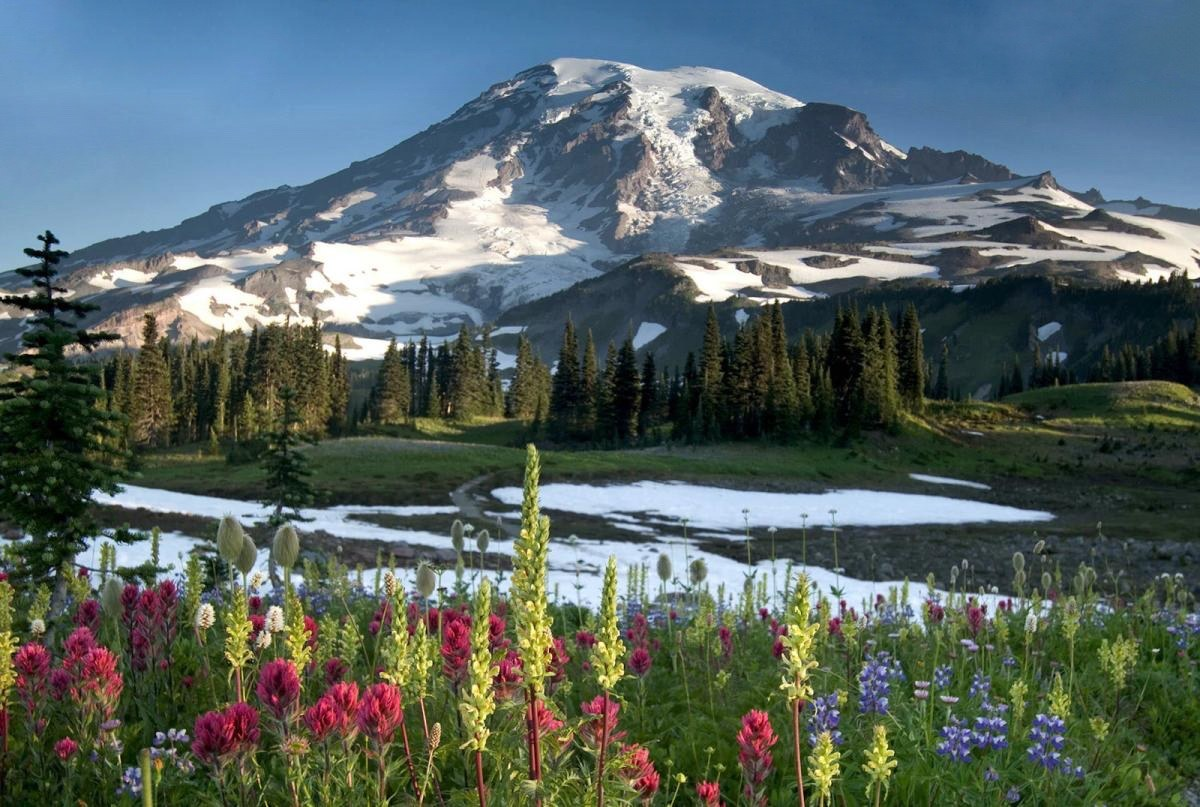
\includegraphics[width=\linewidth]{rainier/input.jpg}
    \caption{Input photograph.}
    \label{fig:rainier-photo}
  \end{subfigure}\hfill
  \begin{subfigure}{0.48\linewidth}
    \centering
    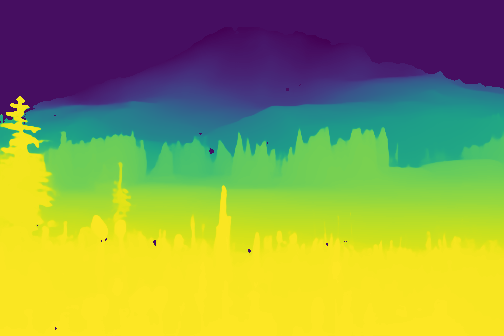
\includegraphics[width=\linewidth]{rainier/depth-perspective.png}
    \caption{Perspective depth, the metric anchor.}
    \label{fig:rainier-depth-persp}
  \end{subfigure}

  \vspace{0.6em}
  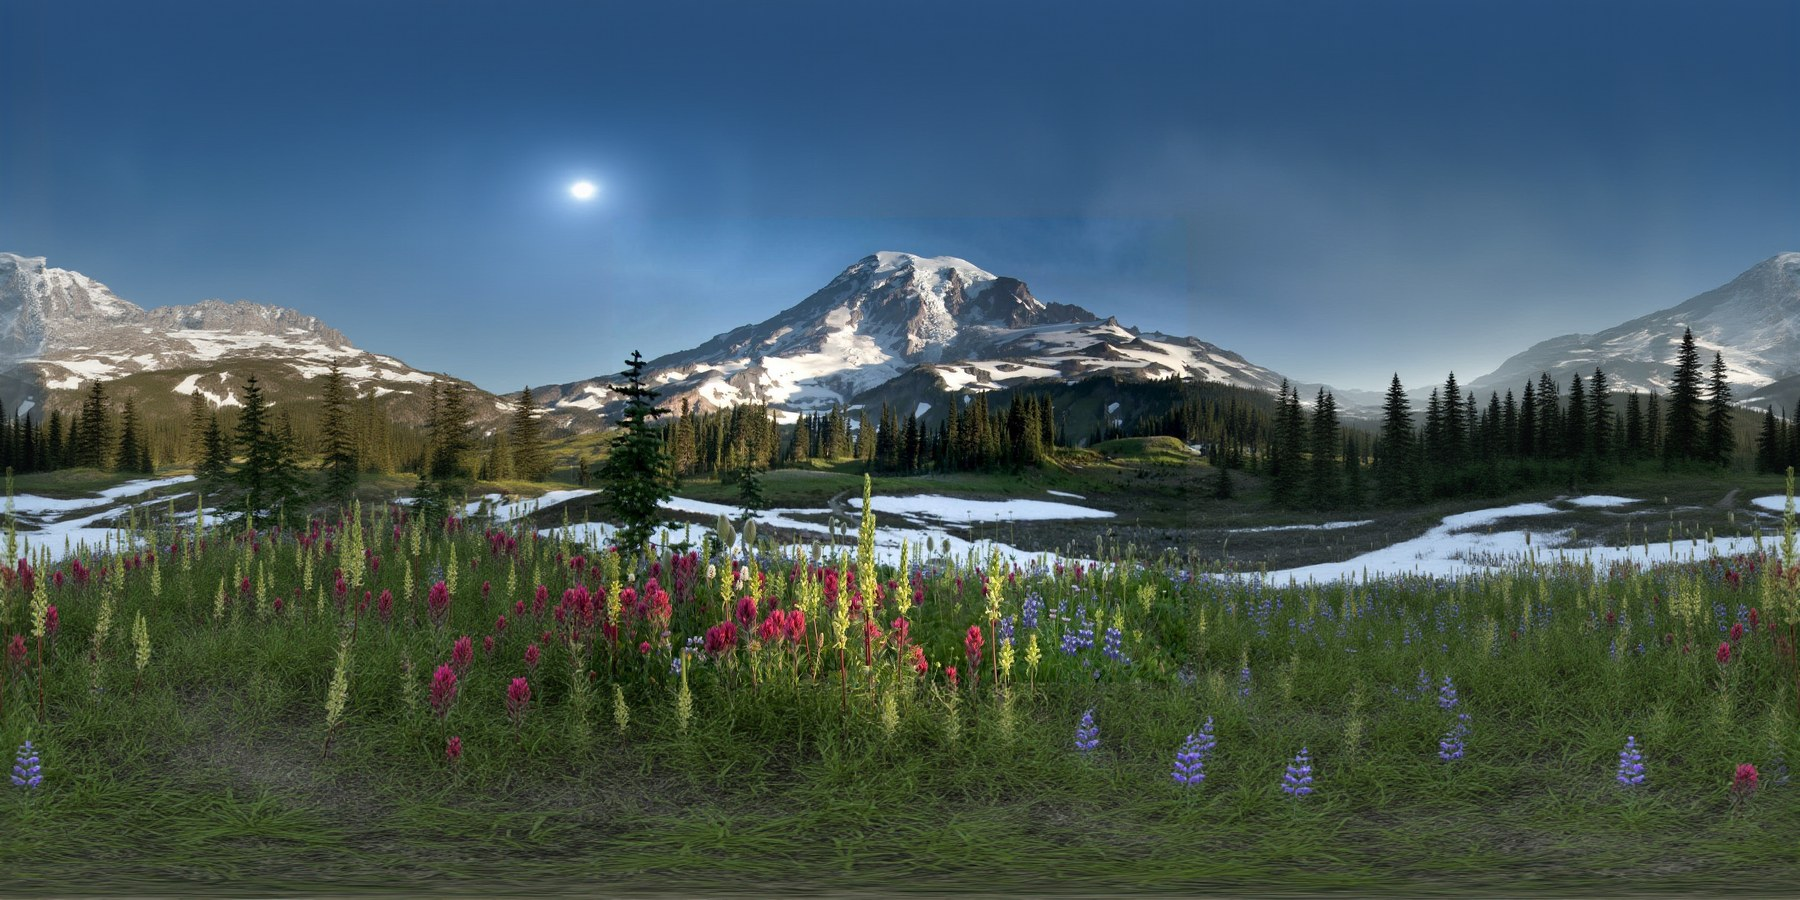
\includegraphics[width=\linewidth]{rainier/panorama.jpg}
  \caption{The Mount Rainier example. The input photograph (a) and its perspective
  depth estimate (b) are outpainted into a full equirectangular panorama (below).
  The photograph occupies the region around the mountain; the remaining
  $\sim$\SI{83}{\percent} of the sphere is generated.}
  \label{fig:rainier-input}
\end{figure}

\subsection{Panorama Generation and Metric Calibration}

The input image is first processed by generating a synthetic caption and a
perspective depth estimate, then outpainting the image to a full equirectangular
panorama, which is super-sampled to its working resolution. Panoramic depth is
estimated on the result~\cite{lin2025dap}.

\emph{Depth Any Panoramas} is built for equirectangular imagery, but its output is
relative rather than metric. We calibrate it against
Depth Anything~3~\cite{lin2025depth3recoveringvisual} run on the original input,
which gives a metric baseline over the region the photograph actually observed.
The two are related by a monotonic response curve rather than a single scale
factor, because the relationship is not linear.

\paragraph{Fitting the response curve.}
Let $r \in [0,1]$ be the panoramic model's raw prediction and $d$ the metric depth
from the perspective model. We project the hero photograph into the panorama using
the same field of view that was used to place it during outpainting, which gives a
set of corresponding samples $\{(r_i, d_i)\}$ over the overlap region. Sky pixels
and non-finite or non-positive samples are discarded. The surviving samples are
partitioned into $N = 14$ quantile bins of $r$, and each bin contributes one knot

\begin{equation}
  c_b = \operatorname{median}\{r_i : i \in \mathcal{B}_b\},
  \qquad
  m_b = \operatorname{median}\{d_i : i \in \mathcal{B}_b\},
\end{equation}

where $\mathcal{B}_b$ is the set of samples in bin $b$. Medians rather than means
keep mismatched samples, typically foreground objects surviving into the overlap,
from dragging a knot, and a running maximum $\tilde{m}_b = \max_{k \le b} m_k$
enforces that depth cannot decrease as the raw prediction increases. Calibration is
attempted only above $300$ valid samples; below that the overlap is too small to fit
reliably and the depth is left uncalibrated. Metric depth is then recovered by
interpolating $(c_b, \tilde{m}_b)$. The curve is treated as a property of the model
rather than of the image, so the same fit applies to every panoramic depth map in
the scene, which is what keeps them on a common scale.

\paragraph{Extrapolating beyond the fitted range.}
The overlap region only ever covers the photograph's own near field, a few to a few
tens of meters, so it never contains genuinely distant terrain. Interpolation alone
would flat-clamp every raw value past the fitted range onto the curve's last knot,
collapsing a mountain a kilometer away and a tree just past the fitted range onto
the same depth. We instead extrapolate in log-depth space, since the raw prediction
approaches its ceiling asymptotically as true depth grows,

\begin{equation}
  d(r) = \exp\!\big(\log \tilde{m}_{N} + s\,(r - c_{N})\big),
  \qquad
  s = \frac{\log \tilde{m}_{N} - \log \tilde{m}_{N-k}}{c_{N} - c_{N-k}},
\end{equation}

with the slope $s$ estimated from the last $k = 3$ knots, and symmetrically at the
near end, capped at $d \le \lambda\,\tilde{m}_N$ with $\lambda = 20$. The cap
matters because the raw output saturates well before true distance does: a
mountainside a few hundred meters out and a hard-clamped sky pixel read at
essentially the same ceiling. A slope estimated from a few tail bins and then
exponentiated over that gap is extremely noise-sensitive, and produced fabricated
depths of tens of kilometers for every pixel sharing a saturated value. One
outlier of that size dominates anything treating panorama depth as a trustworthy
scale, silently discarding real terrain as out of bounds rather than merely far.
The cap recovers no distance the model cannot resolve, but it keeps far content
bounded and ordered.

\paragraph{Fitting the scene into the terrain budget.}
The calibrated map must finally fit inside the terrain grid's footprint,
$D_{\max} = \SI{100}{\meter}$, half the \SI{200}{\meter} grid extent. A uniform
rescale preserves relative distances exactly and is the wrong invariant to protect:
the scale would be set by the most distant thing in the scene, effectively unbounded
for a landscape, and it invalidates the pipeline's second and more load-bearing
anchor, the assumed camera height that places ground at $-h$ below the camera. On
Rainier, fitting a summit kilometers away into \SI{100}{\meter} divided the map by
$6.5\times$: ground \SI{1.37}{\meter} below the camera returned \SI{0.21}{\meter} of
depth, putting the reconstructed surface \SI{0.9}{\meter} \emph{above} eye level
with the camera buried in its own terrain. A flat clamp fails oppositely, collapsing
a \SI{120}{\meter} ridge and a \SI{900}{\meter} peak onto one wall.

We compress only the far end, leaving the near field metrically intact. With a knee
at $k = 0.6\,D_{\max}$ and tail $t = D_{\max} - k$,

\begin{equation}
  d' =
  \begin{cases}
    d, & d \le k, \\[2pt]
    k + t\left(1 - \exp\!\left(-\dfrac{d - k}{t}\right)\right), & d > k.
  \end{cases}
\end{equation}

This is $C^1$ at the knee, strictly monotonic, and asymptotic to $D_{\max}$, so no
pixel exceeds the budget without a hard clamp. Distant content keeps its ordering;
it simply stops being proportional, which it never meaningfully was once a mountain
kilometers away had to fit a \SI{200}{\meter} grid. Because the curve is fixed by
$(D_{\max}, k)$ rather than by the data's maximum, saturated sky cannot contaminate
it, and applying the same function to both depth maps places the same point at the
same distance in each.

\begin{figure}[htbp]
  \centering
  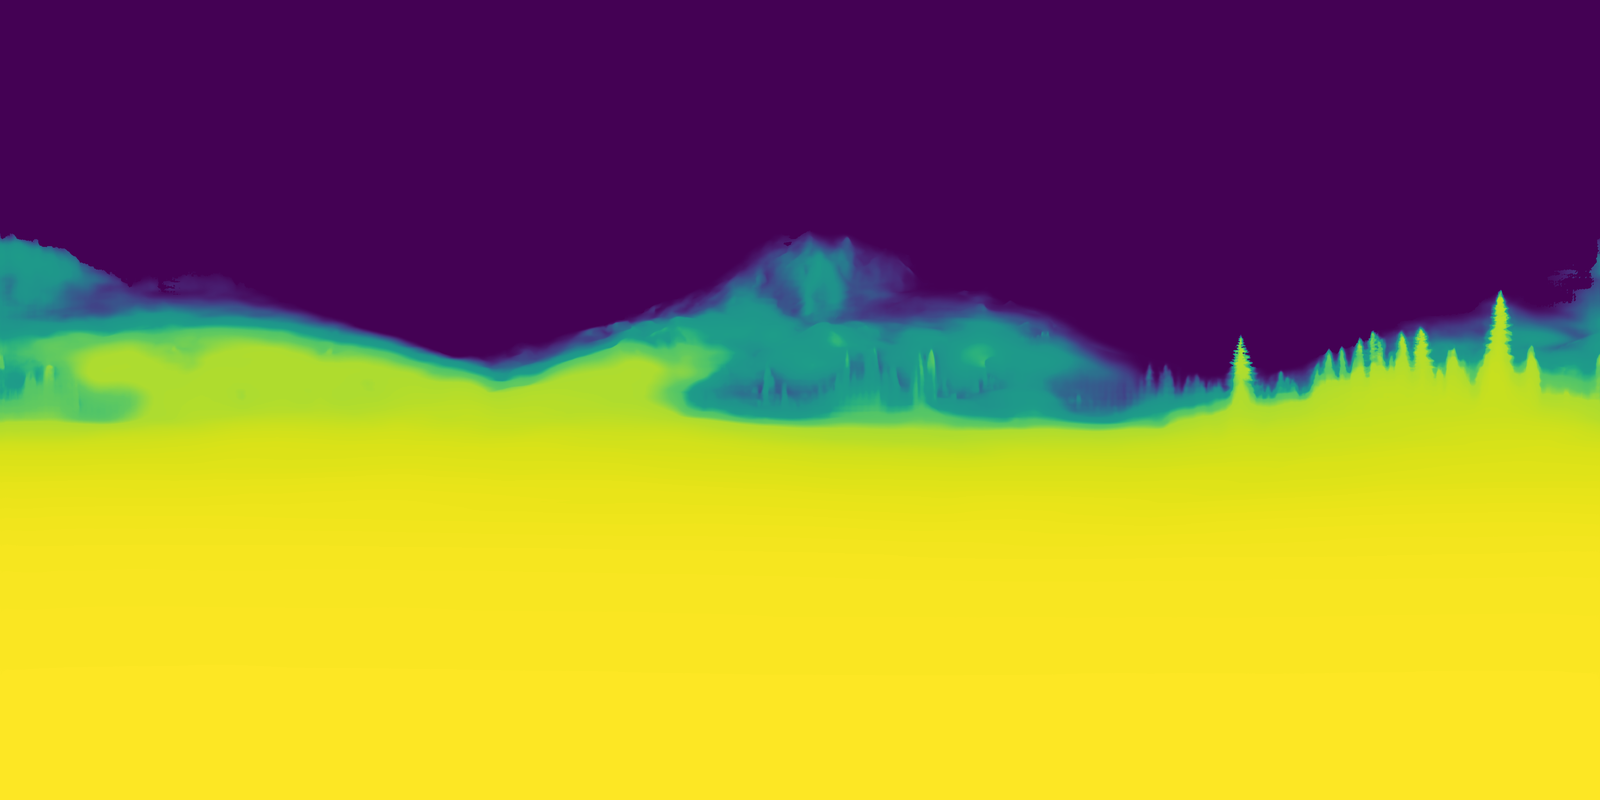
\includegraphics[width=\linewidth]{rainier/depth-calibrated.png}
  \caption{Calibrated panoramic depth for the Rainier capture, near field bright.
  Two properties discussed above are visible directly. The near-field meadow is
  resolved in detail, while everything from the mid-ground treeline outward
  collapses into a narrow band of values: the raw prediction has saturated, and the
  far-range compression maps that whole range onto the approach to
  $D_{\max}$. The sky is masked out rather than assigned a depth.}
  \label{fig:rainier-depth}
\end{figure}

\paragraph{Consequences.}
The result is metrically compressed: near distances are accurate, far ones
systematically shrunk. Since the user explores only a few meters of the scene the
visual effect is minimal, relying on forced perspective, but it is not free.
\Cref{sec:results} returns to a defect it causes, where object size is computed as
angular extent times depth and inherits the same shrinkage.

\subsection{Object-Removed Panorama}

To assist terrain generation we produce a second panorama with foreground objects
removed, using ObjectClear~\cite{zhao2026objectclear}, which removes objects
together with their effects such as reflections and cast shadows. Objects are
selected by depth threshold, taking those closest to the camera.

Depth taken from the panorama with objects still in it produces spurious values and
raised bumps wherever an object stands in front of the ground, since the surface
behind it was never observed; removing them first gives the depth model an
unobstructed view. \Cref{fig:rainier-object-removed} shows the effect: the near-field
meadow dominating the lower half is replaced by the bare ground the terrain track
needs. The edit is destructive by design. The flowers are not discarded but
reconstructed separately as a ground-cover population
(\cref{sec:distribution}), and the region typing that places them is read from the
\emph{original} panorama.

\begin{figure}[htbp]
  \centering
  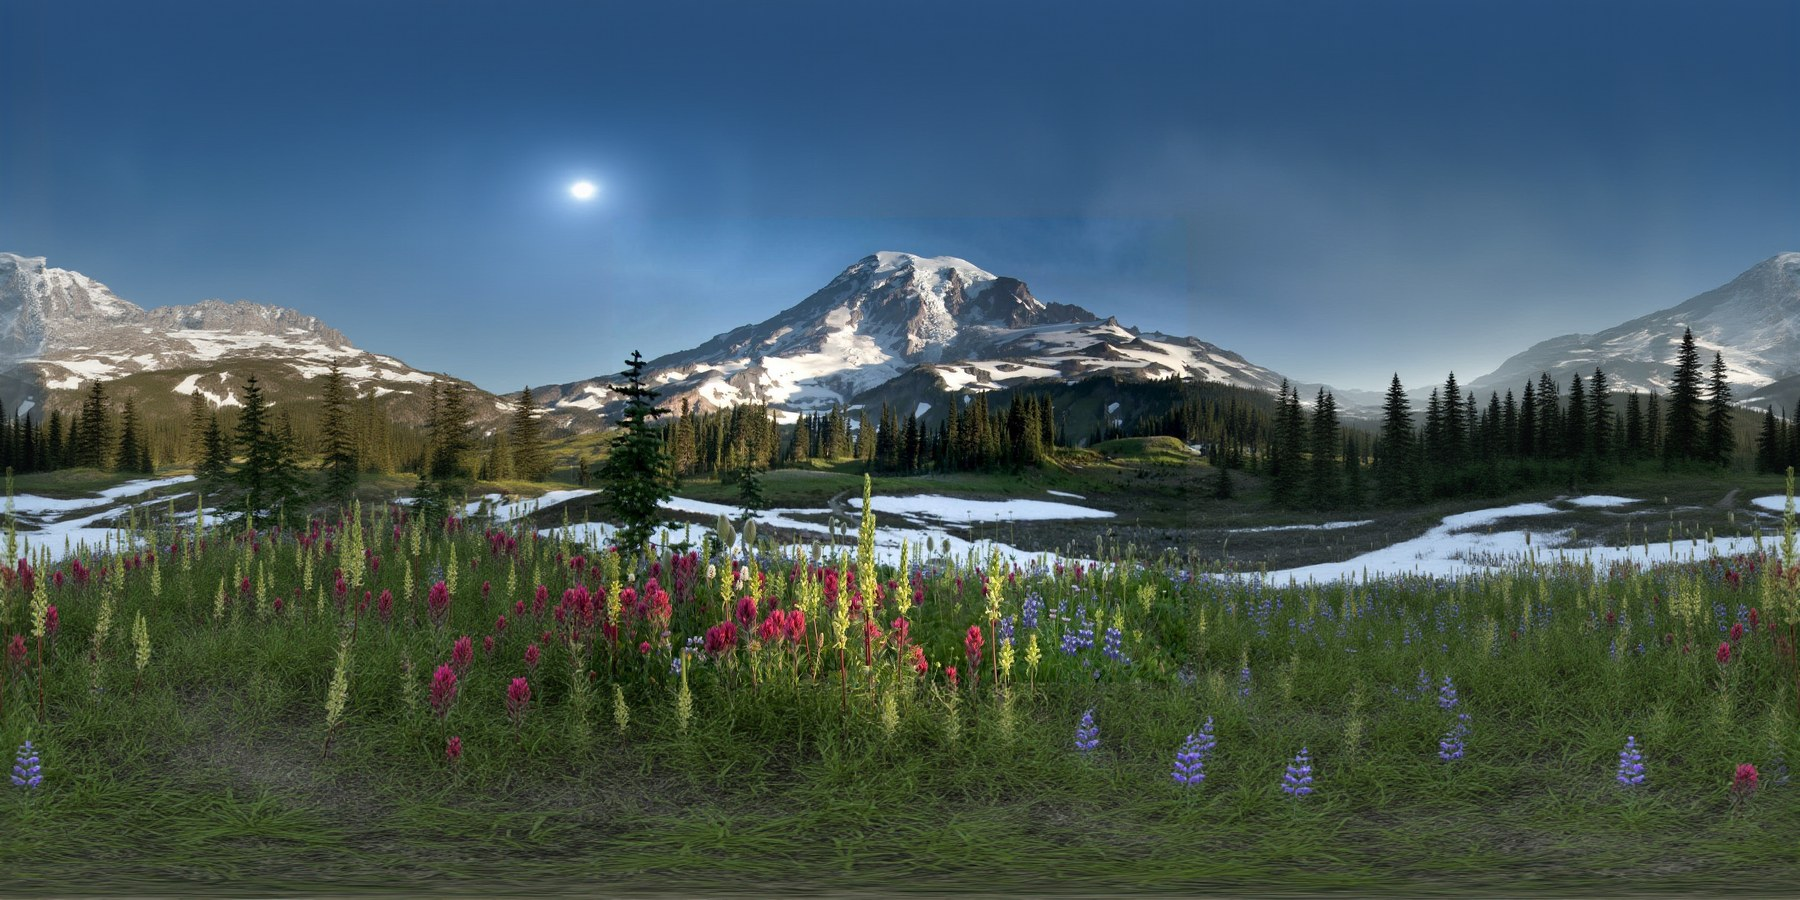
\includegraphics[width=\linewidth]{rainier/panorama.jpg}\\[0.4em]
  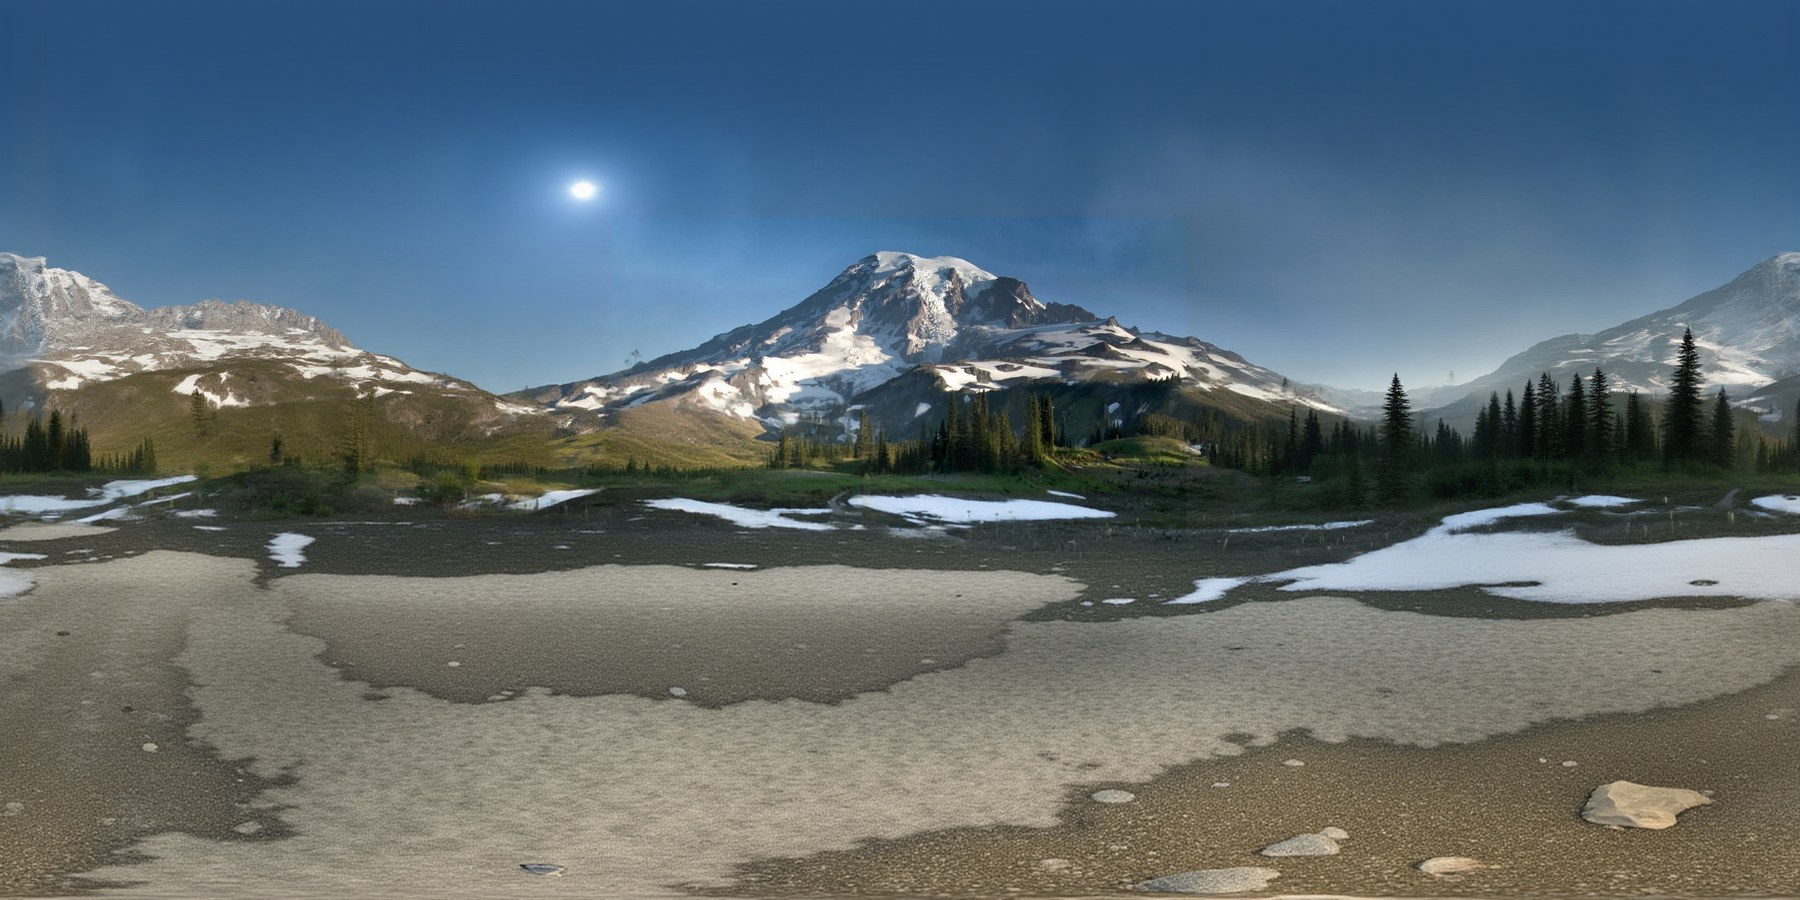
\includegraphics[width=\linewidth]{rainier/panorama-object-removed.jpg}
  \caption{Foreground removal. The original panorama (top) and the object-removed
  panorama (bottom) used for terrain reconstruction. The near-field meadow and the individual
  trees have been removed together with their shadows, exposing the ground surface
  behind them. Depth taken from the top image would place the flower canopy, not the
  ground, at the bottom of the height field.}
  \label{fig:rainier-object-removed}
\end{figure}

\subsection{Semantic Region Map}

SegFormer~\cite{DBLP:journals/corr/abs-2105-15203} assigns per-pixel region types
(sky, water, terrain, ground, vegetation, built objects, road, trail) over the
panorama. This map drives much of the downstream scene understanding, from terrain
construction to object placement.

\begin{figure}[htbp]
  \centering
  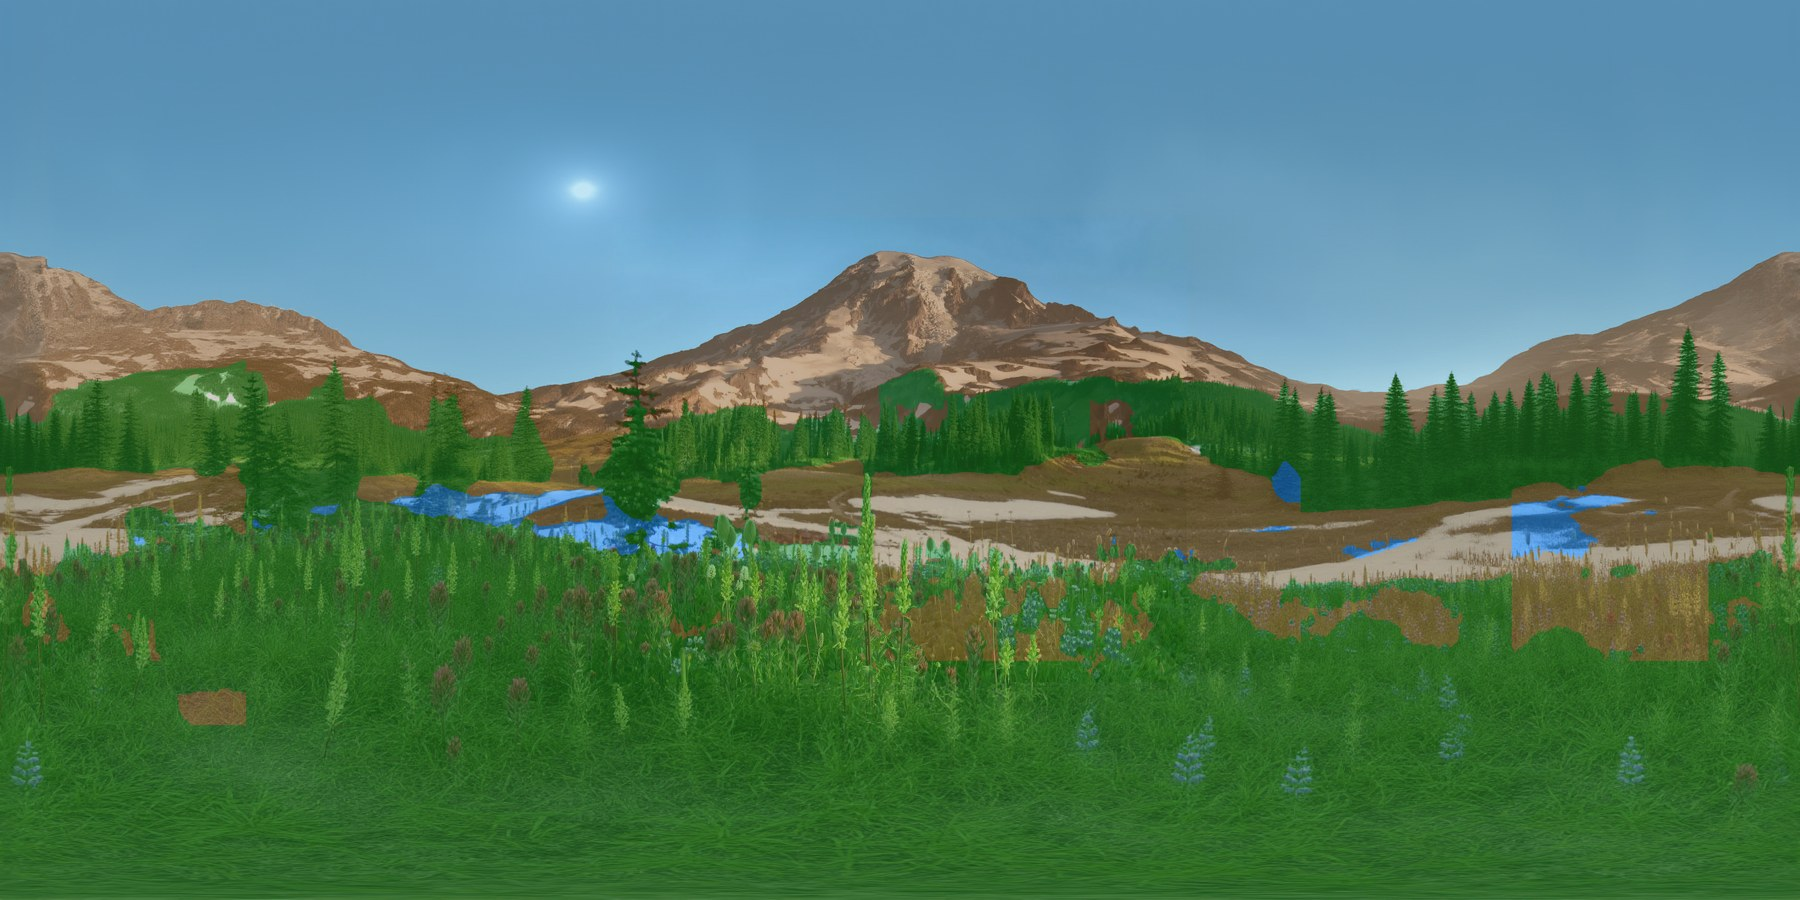
\includegraphics[width=\linewidth]{rainier/regions.jpg}
  \caption{Resolved semantic region typing for the Rainier capture, overlaid on the
  panorama. Vegetation, bare terrain, snow and standing water separate cleanly in
  the near field. The typing is run twice, once on the original panorama and once on
  the object-removed one, because the two answer different questions: where ground cover
  should be scattered is a property of the scene as photographed, while what the
  terrain surface is made of is a property of the scene with the objects taken away.}
  \label{fig:rainier-regions}
\end{figure}

% =============================================================================
\section{Terrain Geometry}
\label{sec:terrain}
% =============================================================================

\subsection{Projection with UV retention}
\label{sec:uv-retention}

The height field is a $4096^2$ top-down grid spanning \SI{200}{\meter}. Each
panorama pixel below the horizon is unprojected to a 3D point using calibrated
depth and accumulated into the grid cell containing its $(x,z)$.

The contribution here is what is retained alongside the height. For every cell
that receives a genuine measurement we store the panorama $(u,v)$ it was observed
through, together with a mask distinguishing directly measured cells from those
later filled by interpolation. This costs two float channels and removes an entire
class of error.

The alternative --- re-deriving $(u,v)$ from the final geometry --- is what a
naive implementation does, and it fails in a specific way. The elevation angle of
a ground point is $\varphi = \arcsin(y/d)$, so near the nadir a small error in $y$
produces a large error in $\varphi$ and therefore in panorama row. Since $y$ has
by then passed through reconstruction, erosion and meshing, it is not the value
that was measured. Retaining the observed UV means downstream texturing samples
the correspondence that was actually observed.

\subsection{Constrained harmonic completion}

The projected height field is sparse and uneven: dense near the camera, sparse at
range, and empty wherever an object occluded the ground. Completion is posed as a
constrained boundary-value problem. Cells with direct, high-certainty measurements
become Dirichlet boundary conditions; distant ridge anchors extracted from the sky
silhouette are added as further fixed values; the remainder is solved as a
discrete harmonic problem
\begin{equation}
  \nabla^2 h = 0 \quad \text{on } \Omega_{\text{unknown}},
  \qquad h = h_{\text{obs}} \quad \text{on } \partial\Omega_{\text{obs}},
\end{equation}
using a sparse linear solve. Measured terrain is therefore never modified, and
unobserved terrain is the smoothest surface consistent with it.

\subsection{Ridge anchoring and its assumption}

Terrain beyond depth range has no usable measurement, so its elevation comes from
the sky boundary: for each panorama column, the first non-sky pixel below sky
gives an elevation angle, placed at a fixed radius on the grid. This is a
deliberate scale compromise --- a mountain kilometres away cannot be walkable
terrain in a \SI{200}{\meter} grid, so it is brought close and shrunk, preserving
silhouette shape rather than true distance.

The assumption embedded here is that the sky boundary is the crest of
\emph{ground}. \Cref{sec:results} shows what happens when it is not.

\subsection{De-spoking}

The equirectangular-to-grid projection maps each panorama column onto a radial
line on the grid. Any per-column bias in the depth prediction therefore becomes a
radial streak, and because those streaks lie in the \emph{observed} data --- around
$89\%$ of solve nodes are fixed --- the harmonic solve cannot remove them.

We remove them with a targeted filter that subtracts only the tangential
high-frequency component, computed as a polar round-trip difference
\begin{equation}
  h' = h - \big(P(h) - G_\sigma^{\theta}(P(h))\big),
\end{equation}
where $P$ is the polar resample and $G_\sigma^{\theta}$ an angular Gaussian blur.
Taking the difference cancels the resampling error, which would otherwise bake in
concentric rings: resampling error is around \SI{1.2}{\meter} against a spoke
signal of roughly \SI{0.2}{\meter}. Validated end-to-end, the radial elevation
profile is unchanged (\SI{18.1}{\meter}/\SI{30.7}{\meter}/\SI{21.8}{\meter} at
$r=45/60/\SI{80}{\meter}$ against \SI{18.1}{\meter}/\SI{30.7}{\meter}/%
\SI{21.9}{\meter} before), the cliff mask is bit-identical, and the mean absolute
change is \SI{0.19}{\meter} concentrated in the spoke regions.

\subsection{Erosion refinement}

Harmonic completion is smooth by construction, which is correct as an estimator
and wrong as terrain. Real landforms carry drainage structure. We therefore run
fluvial incision over the completed field using
Landlab~\cite{barnhart2020landlab,hobley2017creative}, restricted to unobserved
cells so measured ground is preserved. Erosion strength is modulated by a
jaggedness map derived from the ridge silhouette, so the invented relief matches
the character of the visible terrain.

\subsection{Meshing}

The height field is triangulated by Poisson-disc sampling with a near-camera
density bias, then Delaunay triangulation, giving natural level-of-detail without
axis-aligned artefacts. Water regions are extracted as a separate surface, and the
terrain beneath is depressed so an animated water plane never clips through its
bed. Disconnected landmasses above a plausibility threshold are extracted as
separate formation meshes. A coarser collision mesh is generated by the same
procedure with sparser parameters.

Each vertex carries a second UV channel holding the retained panorama coordinate
from \cref{sec:uv-retention}. Because that channel is per-vertex and interpolated
across triangles, triangles spanning an occlusion boundary --- where grid-adjacent
vertices observed very different panorama rows --- smear a wide band of image
across a small piece of ground. We detect these geometrically, comparing each
triangle's UV span against the span its own size and distance predict, and collapse
the offending corner. Detection must be geometric rather than a fixed pixel budget,
because a near triangle legitimately spans tens of degrees while the same triangle
at range spans under two.

% =============================================================================
\section{Terrain Appearance}
\label{sec:texture}
% =============================================================================

\subsection{Why projection alone fails}

The obvious way to texture the ground is to project the panorama onto it. This
fails in two distinct ways.

First, \emph{grazing incidence}. Equirectangular rows compress with distance: at
\SI{80}{\meter} a single panorama row covers roughly \SI{12}{\meter} of ground
when the terrain is flat, against \SI{0.5}{\meter} when the horizon is anchored at
its true elevation. The result is radial smearing.

Second, and less obviously, \emph{upright content}. Projecting assumes the image
at elevation $\varphi$ is ground at radius $h/\tan(-\varphi)$. That holds for bare
terrain and fails completely for anything vertical: a \SI{0.5}{\meter} flower spans
a range of elevations, each landing at a different ground radius, so one flower
smears into a streak metres long. Rendered top-down this produces a radial
pinwheel. It is also double-counting, since the same flowers are placed as 3D
instances on top of the ground.

\subsection{Layered splat material}

Texturing is therefore a weighted blend of layers. A panorama layer supplies real
photographic colour where projection is trustworthy, gated by a visibility weight
that falls off near the nadir and the horizon and is withheld where a texel's own
panorama pixel is vegetation or built structure rather than ground. Synthetic
material layers, generated per region type, supply the rest.

\subsection{Real-material pattern texturing}

Where the panorama layer is withheld, we prefer real material over generated
material. Following pattern-based texturing~\cite{neyret:inria-00537511}, small
reference patches are extracted from the most solid interior of each region in the
panorama and flattened --- by fitting a local plane to the patch's own depth
points and reprojecting, which removes genuine oblique foreshortening rather than
only equirectangular stretch --- then assembled over the mesh's own triangles with
blended borders so the tiling does not read as faceted.

Reference patches are drawn from the object-removed panorama with real ground
colour restored from the original wherever foreground removal ate the ground
rather than an occluder. Where an occluder genuinely was removed, its footprint is
refilled by inpainting from the surrounding real ground, so what remains is
neither the occluder nor fabricated fill.

% =============================================================================
\section{Object Decomposition}
\label{sec:objects}
% =============================================================================

\subsection{Detection, typing and verification}

Objects are segmented on the original panorama with
SAM~2~\cite{ravi2024sam2segmentimages}, tiled and merged to handle equirectangular
distortion. Each crop is classified by CLIP against a fixed category set, with a
BLIP caption~\cite{li2022blipbootstrappinglanguageimagepretraining} as fallback
where the image pass is indeterminate. Labels are then verified by asking
Grounding DINO~\cite{huang2023open} to localise the proposed label in the crop:
CLIP proposes, an independent model disposes.

The reason for verification is that CLIP scores a fixed label set and always
returns a ranking, so on a capture where it has no signal that ranking is
near-uniform noise with a winner. On one alpine capture, of 359 crops the 20 that
survived CLIP's own gates all scored within a $0.019$--$0.034$ top-5 spread: junk
crops and real flowers were numerically indistinguishable.

\subsection{Correlation and clustering}

Surviving detections are grouped by class, then sub-clustered by visual similarity
using DINOv2 embeddings and agglomerative clustering, splitting a class into
appearance variants (flower colours, tree species). Bucket counts are bounded, and
undersized buckets folded into their nearest neighbour, because an unbounded
distance cut produces one bucket per instance --- measured at 302 groups on one
capture, each demanding its own reconstruction.

\subsection{Asset generation and level of detail}

One mesh is reconstructed per (class, bucket) group with
SAM~3D~\cite{sam3dteam2025sam3d3dfyimages} and instanced at every member's
position. Two selection decisions matter. The crop fed to reconstruction is chosen
by \emph{resolution} among those passing quality gates, not by classifier score,
because a single-view reconstructor given too few pixels does not return a worse
object but a different one --- a flat sheet. And the mesh-versus-billboard decision
is made on \emph{projected angular size} rather than distance, since distance only
proxies resolvability when every object is the same size.

Reconstructions are validated against their detections before placement: a mesh
too flat in any axis, or whose aspect ratio disagrees with its detection's, is
rejected in favour of a crossed-card or billboard representation.

% =============================================================================
\section{Population Synthesis}
\label{sec:distribution}
% =============================================================================

A detector finds tens of flowers in a meadow that contains thousands. Placing only
what was detected leaves a scene correct everywhere it was measured and empty
everywhere it was not, which reads worse than either extreme: the eye sees the
sampling pattern rather than the meadow.

Two mechanisms fill that gap, and they are deliberately separate because they
answer different questions. Population synthesis asks \emph{where else would
instances of this class be, given where these ones are}. Ground cover asks
\emph{what is the ground made of}, a question with no discrete instances to
generalize from at all.

\begin{figure}[htbp]
  \centering
  \begin{subfigure}{0.42\linewidth}
    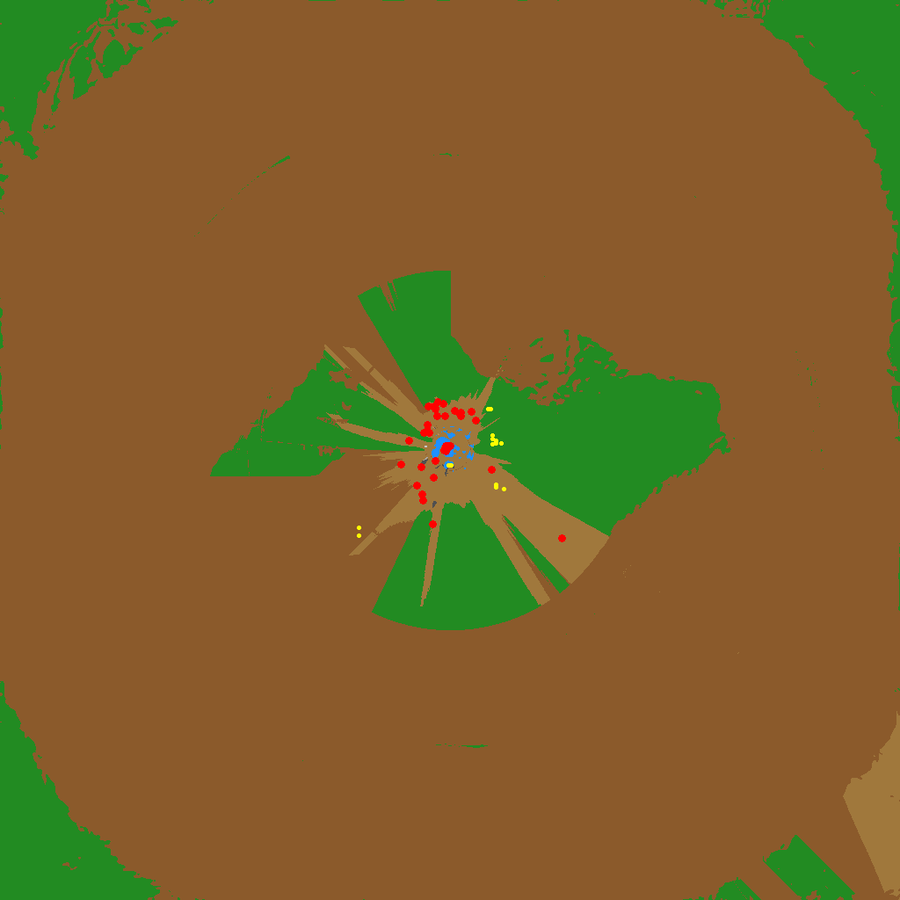
\includegraphics[width=\linewidth]{rainier/synthesis-tree.png}
    \caption{Synthesized tree population.}
    \label{fig:pop-synth}
  \end{subfigure}\hfill
  \begin{subfigure}{0.42\linewidth}
    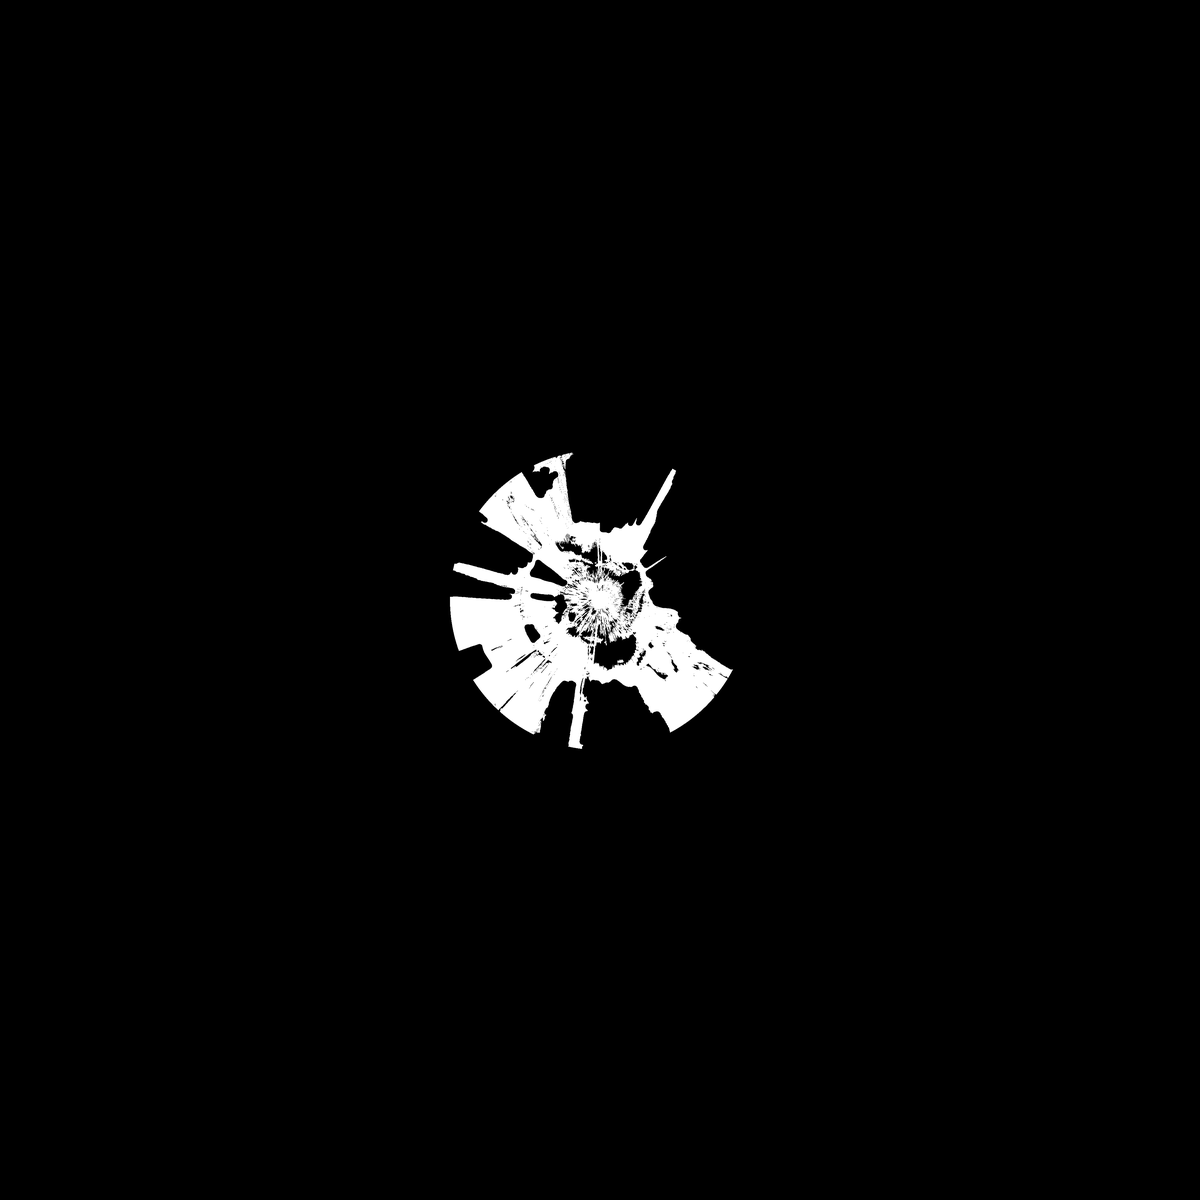
\includegraphics[width=\linewidth]{rainier/grass-area.png}
    \caption{Ground-cover mask.}
    \label{fig:pop-grass}
  \end{subfigure}
  \caption{The two mechanisms on the Rainier capture, both top-down over the
  \SI{200}{\meter} grid. Population synthesis (a) extends the observed tree
  detections outward across the region where that class is admissible, matching
  their measured spatial statistics rather than repeating a fixed density. Ground
  cover (b) is a mask, not a set of instances: it marks where the scattered tuft
  geometry is admissible. The mask is small relative to the grid because it is
  derived from the region typing of the \emph{original} panorama, which only sees
  meadow in the near field the photograph actually observed.}
  \label{fig:rainier-populations}
\end{figure}

\subsection{Synthesis from Observed Statistics}

For each (class, region-type) pair with enough real detections to constitute
evidence, we measure the spatial statistics of those detections as a
pair-correlation histogram, and synthesize additional instances matching them over
the rest of the matching region. This is a point-process
formulation~\cite{9cfc5dfd-c17c-3458-81d1-9c27d3a321e8}, closely related to
appearance-guided element arrangement~\cite{10.1145/1572614.1572623} and in the
spirit of example-based world synthesis~\cite{10.1145/2766975}.

\subsection{Ground Cover}

Grass is not synthesized from detections, because a detector does not usefully
enumerate blades of grass. It is scattered by density over a mask, and the
interesting part is how that mask is derived.

The mask comes from the region typing of the \emph{original} panorama, for the
reason given in \cref{sec:panorama}: the object-removed panorama has had the
meadow erased along with the objects standing in it. But region type alone is too
blunt in a way that matters here. The semantic label set folds \texttt{grass},
\texttt{earth} and \texttt{field} together with \texttt{sand}, \texttt{snow} and
\texttt{ice} into one ground class, so a snowfield and a meadow are
indistinguishable by type, and an alpine meadow is typically ringed by melting
snowpack that types identically to the wildflowers beside it.

Color settles it. Each candidate cell is tested against the excess-green of the
panorama pixel it was observed through, available directly, because that pixel
is the one retained in \cref{sec:uv-retention}. The threshold is deliberately a low
bar rather than a test for lushness: dry grass sits near zero on this scale while
sand runs about $-0.12$ and snow lower still, so it removes only surfaces that are
definitively not vegetation. The same measurement is then reused as a
\emph{weight} rather than a veto, so density tracks how green the ground actually
is instead of being uniform over whatever survives the threshold.

Tufts are placed as fixed-orientation crossed cards rather than camera-facing
billboards. A billboard is a single quad that turns to face the viewer, which
works for an upright subject at eye level and collapses to a line, then swings
through the ground plane, for ground cover underfoot.

% =============================================================================
\section{Lighting and Animation}
\label{sec:lighting}
% =============================================================================

The tracks described so far produce geometry and materials. Two things remain
before the result reads as a place rather than a diorama: it has to be lit
consistently, and it has to move.

\subsection{Illumination and De-lighting}

Scene illumination is estimated from the panorama with
LuxDiT~\cite{liang2025luxdit}, which recovers an HDR environment and a dominant
light direction. The client uses both: the environment as an image-based lighting
source, and the direction as a directional light casting the scene's shadows.

\begin{figure}[htbp]
  \centering
  \begin{subfigure}{0.46\linewidth}
    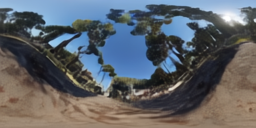
\includegraphics[width=\linewidth]{rainier/lighting-ldr.png}
    \caption{Tone-mapped.}
  \end{subfigure}\hfill
  \begin{subfigure}{0.46\linewidth}
    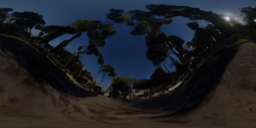
\includegraphics[width=\linewidth]{rainier/lighting-log.png}
    \caption{Log scale.}
  \end{subfigure}
  \caption{Estimated HDR environment for the Rainier capture. The tone-mapped view
  shows what the eye would see; the log view exposes the dynamic range the client
  actually samples, with the sun as a compact high-intensity lobe well above the
  surrounding sky. The dominant direction extracted from this lobe drives the
  scene's directional light.}
  \label{fig:rainier-lighting}
\end{figure}

Estimating the light is only half the problem. Every asset in the scene is cut
from a photograph, so it already carries the illumination of the moment it was
taken: shadows, directional shading, and the color of the light. Rendering
that under a second, freshly estimated light doubles the illumination and the
result reads as flat and over-exposed. Object crops are therefore de-lit with
IntrinsicDiffusion~\cite{Luo2024IntrinsicDiffusion}, which separates albedo from
shading, so what the client relights is material color rather than a photograph.

Two implementation details are worth recording because both are consequences of
the pipeline's structure rather than of the models.

First, de-lighting is applied only to the crops that will actually be rendered, the mesh representatives and the curated billboard
pools, not to every
detection. IntrinsicDiffusion is a diffusion model and the cost is per image; on
a capture with several hundred detections the difference is a substantial
fraction of the total run.

Second, the de-lit image is written under a \emph{new} key rather than replacing
the original crop. Video tracking (below) runs after this stage and matches crops
against a video rendered from the original, fully-lit panorama, so handing the
tracker an albedo image would make it match its own subject worse. Rendering
wants albedo; tracking wants the photograph; both are kept.

\subsection{Motion}

Motion is recovered rather than authored. A short video is generated from the
panorama, each detected object is tracked through it with
SAM~2~\cite{ravi2024sam2segmentimages}, and the resulting trajectory is
classified into a motion type. Category meshes for classes that should move are
then rigged with a sway skeleton, and the client animates them.

Only classes that can plausibly move are tracked, and the per-class tracking
budget is capped. Without a cap the cost is unbounded in a way that is easy to
miss: a single class routinely splits into dozens of appearance buckets, so a
per-bucket limit barely constrains anything: on one capture a ``tree'' class
occupied 65 buckets, most holding one or two instances. Capping per class rather
than per bucket is what makes the stage affordable. Synthesized population points
are excluded entirely; they never appeared in the video, so there is nothing to
track.

\subsection{A Shared Wind Field}

Foliage sway, grass motion and the water surface are driven by one scene-global
wind field rather than by independent per-object oscillators. The field is an
ambient base strength plus discrete gust events, and each point's gust is delayed
by how long the wind takes to physically reach it: distance along the wind axis
divided by gust speed.

That delay is the entire mechanism, and it is what distinguishes a scene that
moves from one that merely wobbles. Independent oscillators produce uniform
agitation everywhere, which reads as noise. A delayed pulse produces a gust that
visibly begins at one side of the scene and sweeps across it, with grass, foliage
and water all responding in step because all three sample the same field. The
water shader evaluates the same gust formula in HLSL that the foliage sway
evaluates in C\#, so the swell rises with the same gust front that bends the
grass.

% =============================================================================
\section{Results and Discussion}
\label{sec:results}
% =============================================================================

\subsection{Evaluation Setup}

We evaluate on three captures chosen to stress different assumptions:
\textbf{Mount Rainier} (alpine meadow, dense vegetation, snow),
\textbf{Paris} (flat urban river scene, architecture), and
\textbf{Shark Fin Cove} (coastal cliffs, open water, sea stacks).

Ground truth 3D does not exist for any of them, so evaluation is necessarily
diagnostic: we instrument the pipeline, measure intermediate quantities against
what the scene demonstrably contains, and localize defects to specific stages.

\begin{figure}[htbp]
  \centering
  \begin{subfigure}{0.5\linewidth}
    \centering
    \figbox{rainier-scene.png}{Mount Rainier: reconstructed scene.}{1.0}
    \caption{Mount Rainier}
  \end{subfigure}

  \vspace{0.9em}
  \begin{subfigure}{0.5\linewidth}
    \centering
    \figbox{paris-scene.png}{Paris: reconstructed scene.}{1.0}
    \caption{Paris}
  \end{subfigure}

  \vspace{0.9em}
  \begin{subfigure}{0.5\linewidth}
    \centering
    \figbox{sharkfin-scene.png}{Shark Fin Cove: reconstructed scene.}{1.0}
    \caption{Shark Fin Cove}
  \end{subfigure}
  \caption{Reconstructed environments viewed from near the capture point.}
  \label{fig:scenes}
\end{figure}

\Cref{fig:scenes} shows three reconstructed environments viewed from near the
capture point.

\subsection{Quantitative Summary}

\Cref{tab:results} summarizes scene composition. The mesh/card/billboard split
indicates how far object reconstruction got on each capture, with the caveat that
the card column is dominated by ground cover rather than by object fallbacks.

\begin{table}[t]
\centering
\small
\caption{Scene composition per capture. \emph{Relief added} is the elevation range
introduced by terrain reconstruction beyond what the height field measured.}
\label{tab:results}
\begin{tabular}{@{}lrrrrl@{}}
\toprule
\textbf{Capture} & \textbf{Meshes} & \textbf{Cards} & \textbf{Billboards} &
\textbf{Relief added} & \textbf{Dominant limitation} \\
\midrule
Mount Rainier   & 128 & 9\,303 & 33 & \SI{35}{\meter} & Conifer reconstruction \\
Paris           & 27  & 4      & 56 & \SI{78}{\meter} & Skyline read as landform \\
Shark Fin Cove  & 0   & 1      & 42 & \SI{81}{\meter} & Detections are rock fragments \\
\bottomrule
\end{tabular}
\end{table}

\subsection{What the Measurements Support}

Two behaviors are worth stating separately from the corrective measures, which
\cref{tab:fixes} quantifies in full.

\paragraph{Terrain geometry on landform scenes.}
Where the horizon genuinely is terrain, reconstruction behaves as intended:
measured cells are preserved exactly by construction, the harmonic solve produces a
continuous surface, and erosion supplies drainage-consistent relief. Mount
Rainier's \SI{35}{\meter} of added relief lies beyond depth range, where the
silhouette is the only evidence available and $98\%$ of it types as terrain.

\paragraph{Ground-cover masking.}
Color vetoing excludes snowfields, which type identically to meadow under the
semantic label set. With the veto ordered after morphological closing, zero grass
instances remain on cells it rejected.

\subsection{Failure Modes and Their Causes}

The more instructive result is where the system fails, because in every case we
localized the failure to an \emph{assumption} rather than a model. A defect can
also surface far from its cause: object size compression originates in depth
calibration (\cref{sec:panorama}) and manifests at placement, eight stages later.
\Cref{sec:remediation} reports what each corrective measure achieved.

\begin{figure}[t]
  \centering
  \figbox{paris-terrain.pdf}{Paris height field before and after reconstruction.}{0.92}
  \caption{The Paris failure. \textbf{Left:} the measured height field, spanning
  \SI{-6.0}{\meter} to \SI{-0.2}{\meter}: correctly flat, and near-featureless
  under a shared shading scale. \textbf{Right:} after ridge-anchored reconstruction,
  spanning \SI{-13.1}{\meter} to \SI{+70.9}{\meter}. Hill \textsf{A}
  (\SI{5966}{\meter\squared}) is the right-bank treeline; hill \textsf{B}
  (\SI{2674}{\meter\squared}) is the cathedral. Both panels share one shading
  scale, so the left panel's flatness is the measurement, not a rendering choice.}
  \label{fig:paris-terrain}
\end{figure}

\paragraph{Skyline read as landform.}
Ridge anchoring assumes the sky boundary is the crest of ground. In Paris it is a
roofline \SI{40}{\meter} away. The measured height field spans
\SI{-6.0}{\meter} to \SI{-0.2}{\meter} (flat, correctly), and reconstruction
produced \SI{-13.1}{\meter} to \SI{+70.9}{\meter}: a \SI{5966}{\meter\squared}
hill on the right-bank treeline and a \SI{2674}{\meter\squared} hill on the
cathedral (\cref{fig:paris-terrain}). The discriminator is what the silhouette is \emph{made of}: the fraction
of silhouette columns typing terrain is $0\%$ for Paris against $87\%$, $98\%$ and
$100\%$ for Iceland, Rainier and Shark Fin. Paris is not merely lowest; not one
column of its horizon is a landform (\cref{fig:silhouette}).

\begin{figure}[t]
  \centering
  \figbox{silhouette-composition.pdf}{Terrain share of the sky boundary per capture.}{0.86}
  \caption{What each capture's horizon is made of. The gate at \SI{25}{\percent}
  separates Paris from every landform capture by a wide margin in both directions;
  it is a threshold on evidence the pipeline already computes, not a tuned constant.}
  \label{fig:silhouette}
\end{figure}

\paragraph{Confident misclassification on texture.}
Shark Fin Cove produced 49 detections at median confidence $0.95$; the two
plausibility vetoes of \cref{tab:fixes} later remove 28 of them, and every instance
that survived failed the reconstruction shape gates. The captions are diagnostic: a rock typed
\emph{person} is captioned ``a piece of pizza with bacon on it''; another typed
\emph{aircraft} is ``a giraffe that is flying in the sky''. On captures with weak
image signal the class is derived from the caption ($59\%$ of Shark Fin crops and
$91\%$ of Rainier's), and the captioner describes unparseable texture fluently
and wrongly. These pass label verification, because a tight cutout fills its own
box and an open-vocabulary detector will localize almost any label inside it.

The consequence for reconstruction is direct: SAM~3D given a flat rock fragment
returns a flat sheet (normalized extents $[1.00, 0.049, 0.425]$), the shape gates
correctly reject it, and every instance falls back to a billboard. Shark Fin's zero
meshes are the gates behaving as intended on inputs that are not objects.

The signal that separates them is the region map, because it is the only opinion in
the chain that does not look at the crop. A per-crop plausibility veto, a class
that cannot occupy the region its box sits in, removes $43\%$ of Shark Fin's
detections with no false positives across the other captures.

\paragraph{Thin vegetation reconstruction.}
Conifers fail single-view reconstruction. Given a good $120\times326$ crop, SAM~3D
returns a mesh with aspect $3.50{:}1$ against detections at $0.12{:}1$, a
$28\times$ disagreement, so 70 of 75 instances fall back to crossed cards. A thin
conifer offers almost no volume cue from one view. Species-aware
approaches~\cite{lee2024tree} are the natural remedy.

\paragraph{Water surface following terrain.}
Water inherited the terrain height under each of its cells, which is correct only
if the ground under a lake is flat. On Shark Fin one \SI{11872}{\meter\squared}
body of sea spanned \SI{73.5}{\meter} in elevation, with $21.7\%$ of its vertices
more than a meter above the median: the ocean draped up the cliffs.

\begin{figure}[t]
  \centering
  \figbox{texel-density.pdf}{Terrain texel density by distance ring.}{0.86}
  \caption{Texture resolution against distance, log scale. The two captures are
  indistinguishable within \SI{25}{\meter}; beyond it Shark Fin degrades far
  faster, because a clifftop camera places most of its surface near the horizon
  where equirectangular compression is worst. Above roughly
  \SI{0.5}{\meter} per texel we take the ground to read as smeared.}
  \label{fig:texel}
\end{figure}

\paragraph{Far-field texture resolution.}
Even with folds repaired, $67.8\%$ of Shark Fin's terrain area exceeds
\SI{0.5}{\meter} per texel against $20.9\%$ for Rainier, because a clifftop camera
places most of its surface near the horizon where equirectangular compression is
worst (\cref{fig:texel}).

\subsection{Corrective Measures and Their Measured Effect}
\label{sec:remediation}

Each failure above was addressed by making its implicit premise testable from
evidence already computed elsewhere in the pipeline, rather than by tuning a
threshold or replacing a model. \Cref{tab:fixes} reports the measured effect of
each, evaluated by replaying the modified stage over saved pipeline state from all
five captures. We report effects on \emph{every} capture, not only the one that
motivated the change, because the risk being managed is regression on scenes that
were already correct.

\begin{table}[t]
\centering
\small
\caption{Corrective measures, the premise each makes testable, and measured effect
across captures. ``FP'' denotes false positives: correct content wrongly removed.}
\label{tab:fixes}
\begin{tabular}{@{}p{3.3cm}p{4.5cm}p{6.2cm}@{}}
\toprule
\textbf{Measure} & \textbf{Premise made testable} & \textbf{Measured effect} \\
\midrule
Silhouette composition gate &
``The sky boundary is the crest of ground'' &
Terrain-typed silhouette fraction: Paris $0\%$; Iceland $87\%$; Rainier $98\%$;
Shark Fin $100\%$. Ridge anchoring suppressed on Paris only; other captures
bit-identical. \\
\addlinespace
Per-crop region plausibility &
``This class can occupy the region its box sits in'' &
Removes 9/109 (Paris), 4/237 (Rainier), 12/49 (Shark Fin), 5/101 (Iceland).
0 FP; Rainier's four are phantom aircraft inside the snowfield. \\
\addlinespace
Caption--scene plausibility &
``The caption describes something this scene can contain'' &
Removes a further 16 (Shark Fin), 16 (Iceland), 9 (Rainier), 2 (Paris). 0 FP.
Requires four conjunctive conditions; each weaker variant deletes real content
(see text). \\
\addlinespace
Water surface levelling &
``The ground beneath water is flat'' &
Shark Fin elevation spread \SI{73.5}{\meter} $\rightarrow$ \SI{0.00}{\meter};
resulting shoreline discontinuity \SI{0.14}{\meter}. Paris (already near-level)
\SI{1.67}{\meter} $\rightarrow$ \SI{0.55}{\meter} across 12 bodies. \\
\addlinespace
Projected-size LOD &
``Distance predicts resolvability'' &
Rainier meshed instances $545 \rightarrow 296$; triangles
\SI{4.47}{M} $\rightarrow$ \SI{2.48}{M}; per-class override table eliminated. \\
\addlinespace
Resolution-based asset selection &
``The best-scoring crop is the best reconstruction input'' &
Source crop area increased $1.0$--$9.2\times$ per group; \num{205} of \num{471}
instances had been rejected as degenerate reconstructions. \\
\addlinespace
Geometric UV-fold repair &
``Adjacent grid cells observed adjacent panorama rows'' &
Collapses \num{5624} triangles (Rainier, $7.0\%$), \num{2169} (Shark Fin),
\num{1479} (Paris). Converges in two passes; face count unchanged. \\
\addlinespace
Occluder-footprint inpainting &
``What foreground removal left behind is ground'' &
Below-horizon pixels showing fabricated fill: $23.9\% \rightarrow 17.1\%$. \\
\bottomrule
\end{tabular}
\end{table}

Two of these deserve comment because the obvious version of each is measurably
wrong.

\paragraph{Caption plausibility requires conjunction.}
Rejecting a detection because its caption mentions something implausible is
appealing and unsafe. On Mount Rainier, 21 flower detections carry captions such as
``a close up of a flower in a vase'', and \num{19} of those \num{21} are real,
placed flowers. The captioner identifies the \emph{subject} correctly and
confabulates the \emph{setting}. Conversely, rejecting on scene-tag support alone
is also unsafe: Rainier's tags name no tree, and it has \num{67} real ones. Only
the conjunction of four conditions (no scene-tag support, implausible caption
vocabulary, caption not naming the class, and class not vegetation) produced
zero false positives. Notably, the caption--class agreement test is unusable as a
veto (its synonym gaps delete real objects) but safe as an \emph{exemption}, because
a gap then merely retains a spurious detection rather than removing a real one.

\paragraph{Robust estimation must respect sampling density.}
Water levelling initially estimated each body's surface from its mesh vertices.
Because the mesh is Poisson-disc sampled with a near-camera density bias,
\num{4309} of Shark Fin's \num{11366} water vertices lie within \SI{20}{\meter} of
the camera, and the resulting estimate described the cove at the viewer's feet
rather than the sea: \SI{-4.54}{\meter} against a shoreline at
\SI{-0.99}{\meter}. Estimating over the uniform grid instead gives
\SI{-1.13}{\meter} and a \SI{0.14}{\meter} shoreline step. The estimator was
correct; the sample weighting was not.

% =============================================================================
\section{Conclusions and Future Work}
\label{sec:conclusions}
% =============================================================================

\subsection{The Case for a Hybrid Pipeline}

The result we most want to draw out is the shape of the system rather than any
single stage. Into Frame mixes learned models and classical graphics roughly
two-to-one by stage count, and neither part would produce this output alone.

Generative models make the problem tractable at all. Five sixths of the sphere and
the ground behind every object are never observed, and no classical reasoning
recovers content absent from the input. Outpainting, foreground removal,
single-view reconstruction and video generation supply it.

What they do not supply is structure. A generative system asked for a scene returns
something viewable: a panorama, a mesh, a radiance field. It does not return a
collidable surface, a population whose density can be sampled, a water plane
animated separately from its bed, or a mesh with a skeleton in it. Every property
that makes the output walkable rather than watchable comes from the classical side:
a harmonic solve that provably never modifies measured ground, fluvial incision,
point-process synthesis fitted to observed statistics, pattern texturing, and a
three-bone rig driven by a shared wind field. Of the 38 active stages, 12 use no
learned model at all, and those are disproportionately the ones producing physical
behavior.

The division of labor is the point. Learned components answer \emph{what is there},
including where nothing was observed; classical components decide \emph{how it
behaves}, under constraints a generative model cannot honor: measured terrain must
survive completion unchanged, water must sit below its bed, a meadow of thousands
of plants must remain one instanced draw. Treating those as requirements rather
than as things to be learned is what turns a picture of a place into a place.

It also explains our failures. As \cref{sec:results} sets out, the surviving defects
are mostly not model failures but assumption failures, where a step correct for one
scene category is applied silently to another. That is the more tractable problem:
an assumption can be identified, measured, and gated.

\subsection{Future Work}

\paragraph{Explicit scene classification.} A first-class scene-type estimate
(natural landform, urban, coastal, interior) consumed by every stage that
currently embeds an implicit assumption would address the largest class of failure
we observed. The system is biased toward outdoor natural scenes, and several
assumptions do not hold outside them: that the sky boundary is the crest of ground,
that a large uniform region is terrain, that vegetation is the dominant content.

\paragraph{Confidence propagation.} Stages produce point estimates. Propagating
uncertainty would let downstream stages weigh evidence rather than accept it, and
would let the system report where it is guessing.

\paragraph{Better single-view reconstruction for thin structures.} Vegetation is
the dominant content of natural scenes and the weakest part of our object track;
species-aware priors~\cite{lee2024tree} are the obvious direction.

\paragraph{Joint refinement.} The pipeline is strictly feed-forward. A closing
optimization that adjusted depth, geometry and placement jointly against
photometric consistency could correct compounded error that no single stage can
see.

\paragraph{Perceptual evaluation.} Our evaluation is diagnostic: it measures where
the system is wrong, not how the result feels to be inside. A user study of
presence, scale perception and navigation comfort would test what the system is
actually for, and is the clearest gap in our rigor.

\paragraph{Audio and interaction.} The scene is something to move through rather
than to act on. Spatialized audio generated jointly with the
scene~\cite{jin2026sonoworld}, and ways for the user to disturb the environment
rather than only observe it, would extend interactivity in the direction this
framing implies.

\subsection{Closing Remarks}

Into Frame demonstrates that a single photograph can become an interactive
environment, with terrain, objects, ground cover, water and lighting reconstructed
as distinct physical components rather than as one representation serving every
purpose. That decomposition buys the depth of the result: each component is
reconstructed by a method suited to its role and then behaves according to it.

The remaining failures are mostly not failures of any model, but assumptions that
held for outdoor natural landscapes and did not extrapolate beyond them. That is an
encouraging place to stop: the boundaries are legible and measurable, and addressing
them means making implicit commitments explicit rather than waiting for better
models.


% =============================================================================
{\small
\bibliographystyle{plain}
\bibliography{references}}
% =============================================================================

\end{document}
